\documentclass{article}
\usepackage{wallpaper}
\usepackage[a4paper,left=0cm, right=0cm, top=0cm, bottom=0cm, outer=0cm, inner=0cm]{geometry}
\usepackage{enumitem}
\usepackage[absolute,overlay]{textpos}
\usepackage{xfp}
\usepackage{tikz}
\usetikzlibrary{shapes.misc}
\usepackage[dvipsnames]{xcolor}

\setlength{\TPHorizModule}{1cm} % Set horizontal unit
\setlength{\TPVertModule}{1cm}  % Set vertical unit

\newcommand{\themecolor}{MidnightBlue}
\newcommand{\subthemecolor}{white}

%Syntax: <color> <x> <y>
\newcommand{\drawcircle}[2]{
\begin{tikzpicture}[overlay]
    \shade[ball color=\themecolor!70!white] (#1,-#2) circle [radius=0.75cm];
\end{tikzpicture}
}

%Syntax: <x> <y> <image path> <title> <text>
%  <x> : x-coordinate (in cm) of image
%  <y> : y-coordinate (in cm) of image
% 
\newcommand{\textblockwithpicture}[5]{ 

  \begin{textblock}{10}(#1,#2)
  \includegraphics[width=1cm,keepaspectratio]{#3}
  \end{textblock}

  \begin{textblock}{10}(\fpeval{2 + #1}, #2)
  \raggedright\Large{\textcolor{\themecolor}{#4}}\\
  \normalsize{#5}
\end{textblock}
}

% Syntax: <x> <y> <title> <picture> <info>
\newcommand{\contactblock}[5]{
%9.5, 24
\begin{textblock}{8}(#1,#2)
\raggedright\Large{\textcolor{\themecolor}{\textbf{#3}}}
\end{textblock}

\begin{textblock}{8}(\fpeval{#1 + 2.25}, \fpeval{#2 - 0.25})
\includegraphics[width=1cm,keepaspectratio]{#4}
\end{textblock}

\begin{textblock}{8}(\fpeval{#1 + 4}, #2)
\raggedright\large{#5}
\end{textblock}
}

\begin{document}
\ThisLRCornerWallPaper{1.1}{background.jpg}
\phantom{hi}

\begin{tikzpicture}[overlay]
\shade[rounded corners=0.5cm, shading=axis, left color=\themecolor!90, right color=\themecolor!75, shading angle=45]
      (-1, 1) rectangle (13cm, -7cm);
\end{tikzpicture}

\begin{textblock}{12}(0.5,0.5) 
\raggedright\Huge{\textcolor{\subthemecolor}{JOIN US FOR THE SIMCODES\\
REU PROGRAM IN AMES, IA!}}
\vspace{0.25cm}\\
\Large{\textcolor{\subthemecolor}{June 8, 2026--- July 31, 2026}}
\vspace{0.25cm}\\
\large{\textcolor{\subthemecolor}{SIMCODES --- The Sustainability Institute for Machine learning and 
Collaborative Open-Source Development of Enzymatic Simulations}}
\vspace{0.5cm}\\
\Large{\textcolor{\subthemecolor}{Are you an early career undergraduate interested in cutting-edge research?
Join us at Iowa State University for a
unique, cross-disciplinary opportunity!}}
\end{textblock}

\begin{textblock}{10}(13.5, 0.25)
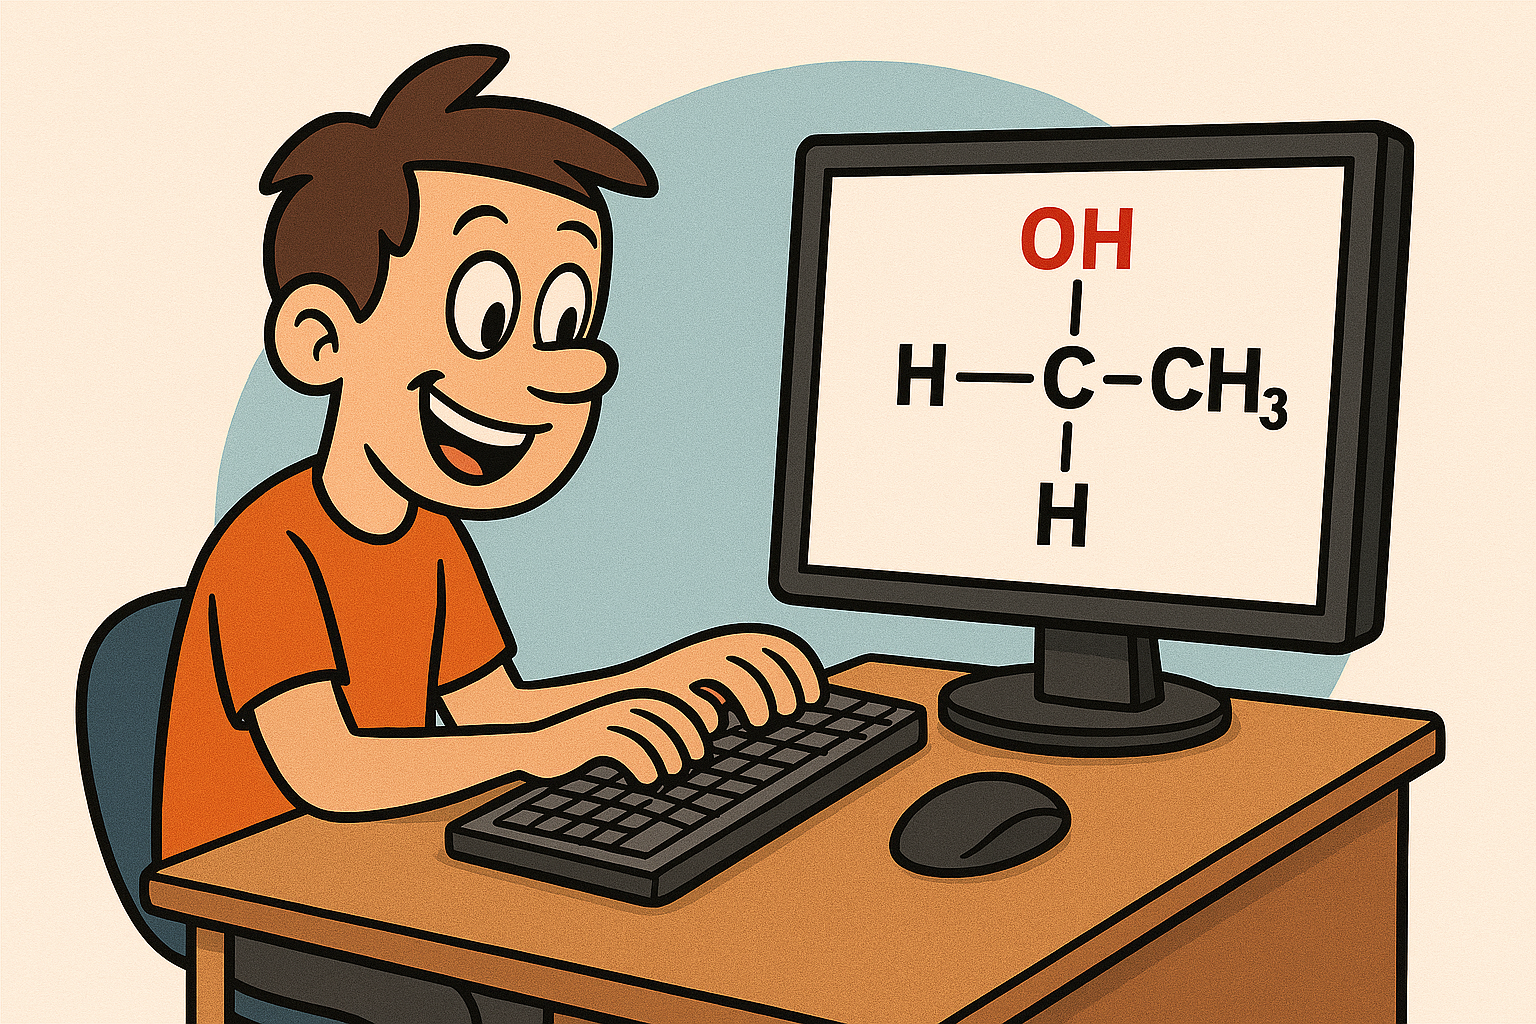
\includegraphics[width=6cm,keepaspectratio]{guy_on_computer.png}
\end{textblock}

\begin{textblock}{10}(13.5, 4.5)
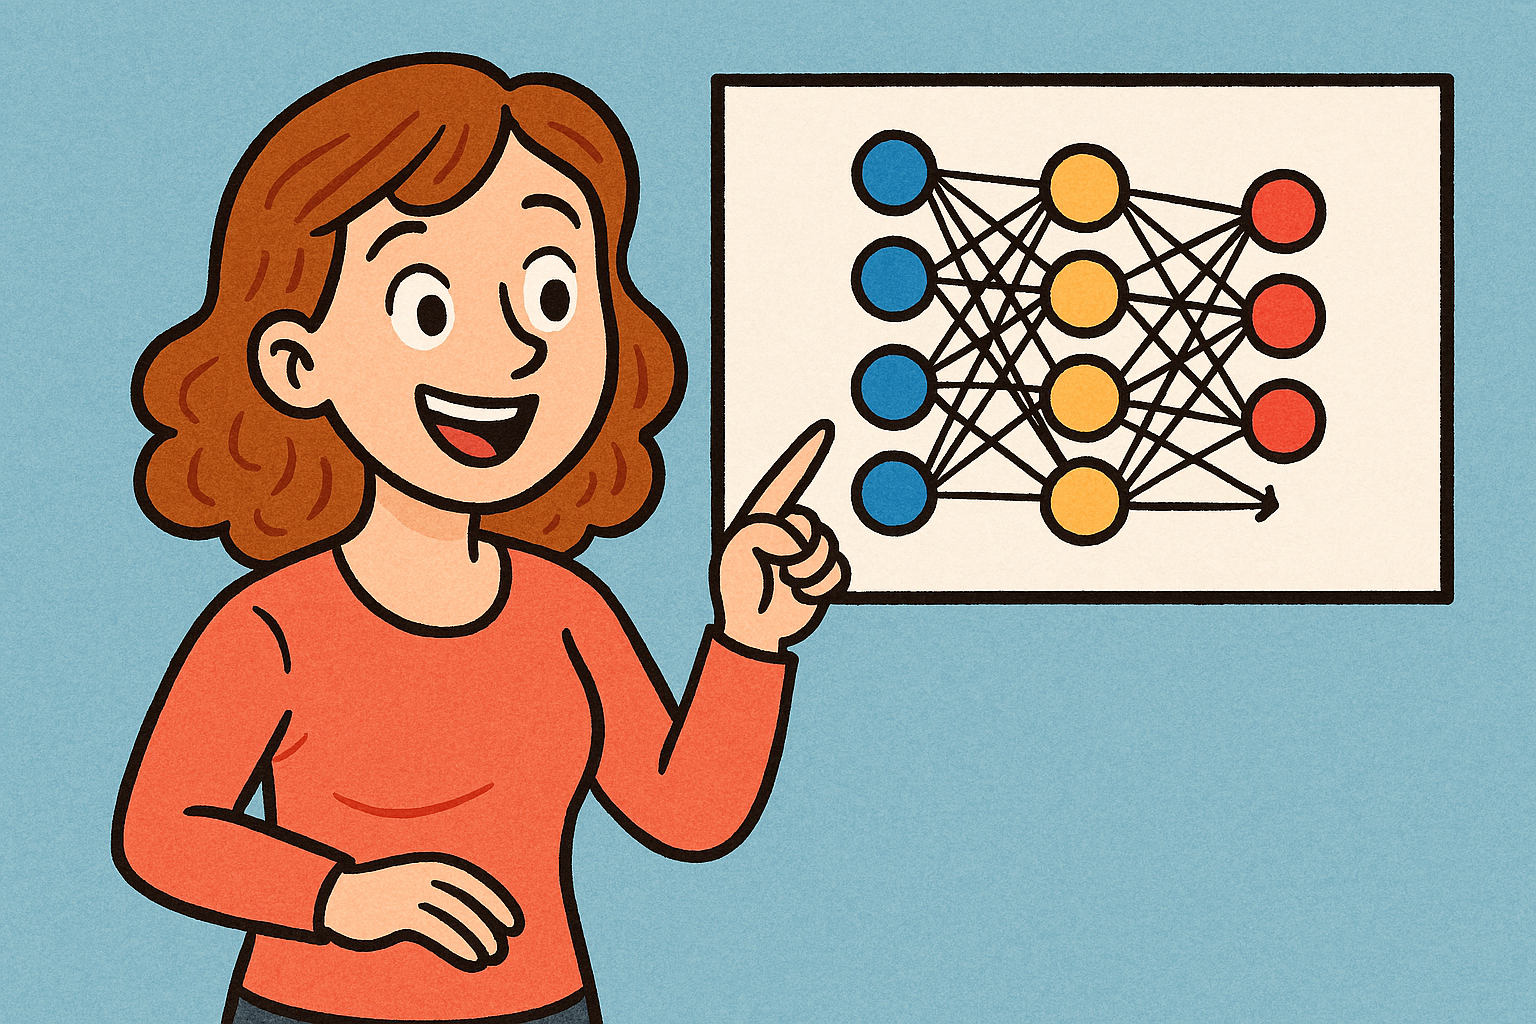
\includegraphics[width=6cm,keepaspectratio]{girl_nn.png}
\end{textblock}

\drawcircle{1}{8.375}
\textblockwithpicture{0.5}{9}{molecule.png}{RESEARCH AREAS}{
Chemistry, Computer\\
Science, Software\\
Engineering, Data Science
}

\drawcircle{1}{11}
\textblockwithpicture{0.5}{12}{flask.png}{HANDS-ON EXPERIENCE}{
Chemistry, Computer\\
Science, Software\\
Engineering, Data Science
}

\drawcircle{1}{13.5}
\textblockwithpicture{0.5}{15}{hammer.png}{WORKSHOPS \& LECTURES}{
Learn state-of-the-art\\
practices in computational\\
chemistry, machine learning,\\
and computer science
}

\drawcircle{10.5}{7.125}
\textblockwithpicture{10}{9}{network.png}{PROFESSIONAL DEVELOPMENT}{
Network, explore career\\
opportunities, resume building,\\
team building
}

\drawcircle{10.5}{9.75}
\textblockwithpicture{10}{12}{microscope.png}{PROJECTS}{
Molecular dynamics\\
simulations, machine learning\\
models, new ML techniques,\\
high-performance algorithms
}

\drawcircle{10.5}{12.25}
\textblockwithpicture{10}{15}{presentation.png}{CAPSTONE PRESENTATION}{
Showcase your research to\\
peers and ISU faculty and staff
}

\begin{tikzpicture}[overlay]
\shade[rounded corners=0.5cm, shading=axis, left color=\themecolor!90, right color=\themecolor!75, shading angle=45]
      (5, -14) rectangle (18cm, -18cm);
\end{tikzpicture}

\begin{textblock}{8}(6,19.5)
\raggedright\Huge{\textcolor{\subthemecolor}{WHY JOIN?}}
\end{textblock}

\begin{textblock}{8}(11,18.25)
\textcolor{\subthemecolor}{
\begin{itemize}[noitemsep]
\item Gain valuable research experience
\item Work with a diverse cohort of students
\item Learn from leading experts in the field
\item Paid 10 week internship including\\
housing, meals, and travel.
\item Stipend - \$7000
\end{itemize}
}
\end{textblock}

\begin{textblock}{8}(0.5,21.25)
\raggedright\huge{\textcolor{\subthemecolor}{Apply Now!}}
\end{textblock}

\begin{textblock}{8}(0.25,22)

\includegraphics[width=3cm,keepaspectratio]{qr.png}
\end{textblock}

\contactblock{8.5}{22.5}{Website}{link.png}{https://simcodes-isu.github.io}
\contactblock{8.5}{24}{Questions?}{letter.png}{Ryan Richard rrichard@iastate.edu}

\end{document}